\documentclass[pdf,aspectratio=169,14pt]{beamer}
\mode<presentation>{}
\usepackage{listings}
\usepackage{graphicx}
\usepackage{theme/beamerthemecoreos169}

\title{Intro to rkt}
\subtitle{What is rkt and how do I use it?}
\author{Derek Gonyeo}

\graphicspath{ {./images/} }

\begin{document}

\lstdefinestyle{log}{
    basicstyle=\scriptsize\ttfamily
}

\begin{frame}
    \titlepage
\end{frame}

\begin{frame}
    Outline
    \begin{itemize}
        \item What are containers?
        \item What is rkt?
        \item How do I get rkt?
        \item How do I use rkt?
        \item How does rkt compare to docker?
        \item How does rkt work?
        \item How do I build rkt containers?
        \item How does rktnetes work?
    \end{itemize}
\end{frame}

% Section: What are containers

\begin{frame}
    Outline
    \begin{itemize}
        \item \textbf{What are containers?}
        \item What is rkt?
        \item How do I get rkt?
        \item How do I use rkt?
        \item How does rkt compare to docker?
        \item How does rkt work?
        \item How do I build rkt containers?
        \item How does rktnetes work?
    \end{itemize}
\end{frame}

\begin{frame}{What are containers?}
    Linux containers are a way to isolate applications. \\
    \vspace{1em}
    \pause
    They're implemented with:
    \begin{itemize}
        \item The chroot syscall provides a different view of the filesystem
        \item pid namespaces prevent an application from seeing other processes
        \item network namespaces give an application a different network
            interface
        \item mount namespaces let an application have different mounts than
            its host
        \item Also UTS/IPC/cgroup/user namespaces
    \end{itemize}
\end{frame}

\begin{frame}{What are containers?}
    Linux containers are a way to run applications, be it in production or on
    your laptop. \\
    \vspace{1em}
    \pause
    They provide:
    \begin{itemize}
        \item A way to package your applications and their dependencies into an
            image.
        \item An easy way to share these container images between machines (via
            centralized repositories).
        \item A way to run your applications in an isolated and consistent
            environment.
    \end{itemize}
\end{frame}

% Section: what is rkt

\begin{frame}
    Outline
    \begin{itemize}
        \item \textbf{What are containers?}
        \item What is rkt?
        \item How do I get rkt?
        \item How do I use rkt?
        \item How does rkt compare to docker?
        \item How does rkt work?
        \item How do I build rkt containers?
        \item How does rktnetes work?
    \end{itemize}
\end{frame}

\begin{frame}
    Outline
    \begin{itemize}
        \item What are containers?
        \item \textbf{What is rkt?}
        \item How do I get rkt?
        \item How do I use rkt?
        \item How does rkt compare to docker?
        \item How does rkt work?
        \item How do I build rkt containers?
        \item How does rktnetes work?
    \end{itemize}
\end{frame}

\begin{frame}{What is rkt?}
    rkt is the piece of software that can fetch and run container images,
    called a container runtime.

    Specifically, it can:
    \begin{itemize}
        \pause
        \item Fetch container images
        \pause
        \item Store and manage local container images
        \pause
        \item Run a container image
    \end{itemize}
\end{frame}

\begin{frame}{What is rkt?}
    rkt follows the Unix philosophy:
    \begin{itemize}
        \pause
        \item Simple cli interface
        \pause
        \item Has well-defined operations
        \pause
        \item No central privileged long-running components
        \pause
        \item Has separate privileges for different operations
    \end{itemize}
\end{frame}

% Section: how do I get rkt?

\begin{frame}
    Outline
    \begin{itemize}
        \item What are containers?
        \item \textbf{What is rkt?}
        \item How do I get rkt?
        \item How do I use rkt?
        \item How does rkt compare to docker?
        \item How does rkt work?
        \item How do I build rkt containers?
        \item How does rktnetes work?
    \end{itemize}
\end{frame}

\begin{frame}
    Outline
    \begin{itemize}
        \item What are containers?
        \item What is rkt?
        \item \textbf{How do I get rkt?}
        \item How do I use rkt?
        \item How does rkt compare to docker?
        \item How does rkt work?
        \item How do I build rkt containers?
        \item How does rktnetes work?
    \end{itemize}
\end{frame}

\begin{frame}{How do I get rkt?}
    rkt is only available on Linux, for amd64 and arm64. \\
    GitHub releases should work on any system with glibc. \\
    \pause
    \vspace{1em}
    Packaged in:
    \begin{itemize}
        \item CoreOS
        \item Debian
        \item Fedora
        \item Arch
        \item Gentoo
        \item Nix
    \end{itemize}
    \pause
    There's also a \texttt{Vagrantfile} in the rkt repo!
\end{frame}

% Section: How do I use rkt?

\begin{frame}
    Outline
    \begin{itemize}
        \item What are containers?
        \item What is rkt?
        \item \textbf{How do I get rkt?}
        \item How do I use rkt?
        \item How does rkt compare to docker?
        \item How does rkt work?
        \item How do I build rkt containers?
        \item How does rktnetes work?
    \end{itemize}
\end{frame}

\begin{frame}
    Outline
    \begin{itemize}
        \item What are containers?
        \item What is rkt?
        \item How do I get rkt?
        \item \textbf{How do I use rkt?}
        \item How does rkt compare to docker?
        \item How does rkt work?
        \item How do I build rkt containers?
        \item How does rktnetes work?
    \end{itemize}
\end{frame}

\begin{frame}{How do I use rkt?}
    Let's start out with an interactive alpine container: \\
    \texttt{rkt run quay.io/coreos/alpine-sh --interactive}
    %\vspace{1em}
    %\lstinputlisting[style=log]{rkt-alpine.log}
\end{frame}

\begin{frame}{How do I use rkt?}
    \texttt{rkt list} will show you all of your exited and running pods.
    %\vspace{1em}
    %\lstinputlisting[style=log]{rkt-list.log}
\end{frame}

\begin{frame}{How do I use rkt?}
    \texttt{rkt image list} will show you all of your stored images.
    %\vspace{1em}
    %\lstinputlisting[style=log]{rkt-image-list.log}
\end{frame}

\begin{frame}{How do I use rkt?}
    To remove old containers: \texttt{rkt gc} \\
    To remove old images: \texttt{rkt image gc}
\end{frame}

\begin{frame}{How do I use rkt?}
    rkt supports docker images! You can refer to them using the
    \texttt{docker://} prefix. \\
    \vspace{1em}
    \texttt{rkt run docker://ubuntu --interactive --exec=bash} 
\end{frame}

\begin{frame}{How do I use rkt?}
    A non-interactive example... \\
    \vspace{1em}
    \texttt{\noindent
        rkt run coreos.com/etcd:v3.0.3 \\
        rkt list \\
        rkt enter \textit{hash} /etcdctl cluster-health
    }
\end{frame}

\begin{frame}{How do I use rkt?}
    Expected question: ``wait, it's always in the foreground?'' \\
    \pause
    \vspace{1em}
    Answer: yup! Use your init system to manage rkt processes, same as any
    long-running process. \\
    Use Ctrl+] three times to kill rkt.
\end{frame}

\begin{frame}{How do I use rkt?}
    Same example, but with \texttt{systemd-run}: \\
    \vspace{1em}
    \texttt{\noindent
        \pause
        systemd-run rkt run coreos.com/etcd:v3.0.3 --net=host \\
        \pause
        systemctl status \textit{service} \\
        \pause
        journalctl -u \textit{service} \\
        \pause
        machinectl list
    }
\end{frame}

% Section: how does rkt compare to docker?

\begin{frame}
    Outline
    \begin{itemize}
        \item What are containers?
        \item What is rkt?
        \item How do I get rkt?
        \item \textbf{How do I use rkt?}
        \item How does rkt compare to docker?
        \item How does rkt work?
        \item How do I build rkt containers?
        \item How does rktnetes work?
    \end{itemize}
\end{frame}

\begin{frame}
    Outline
    \begin{itemize}
        \item What are containers?
        \item What is rkt?
        \item How do I get rkt?
        \item How do I use rkt?
        \item \textbf{How does rkt compare to docker?}
        \item How does rkt work?
        \item How do I build rkt containers?
        \item How does rktnetes work?
    \end{itemize}
\end{frame}

\begin{frame}{How does rkt compare to docker?}
    \begin{center}
        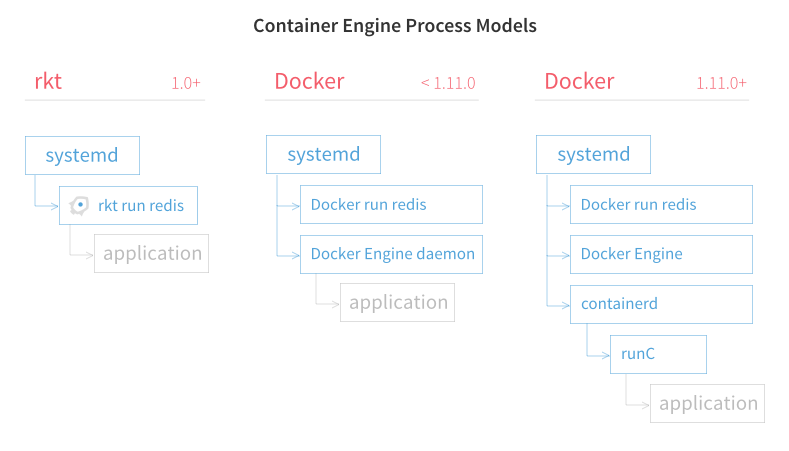
\includegraphics[width=0.75\textwidth]{rkt-vs-docker-process-model}
    \end{center}
\end{frame}

\begin{frame}{How does rkt compare to docker?}
    \begin{center}
        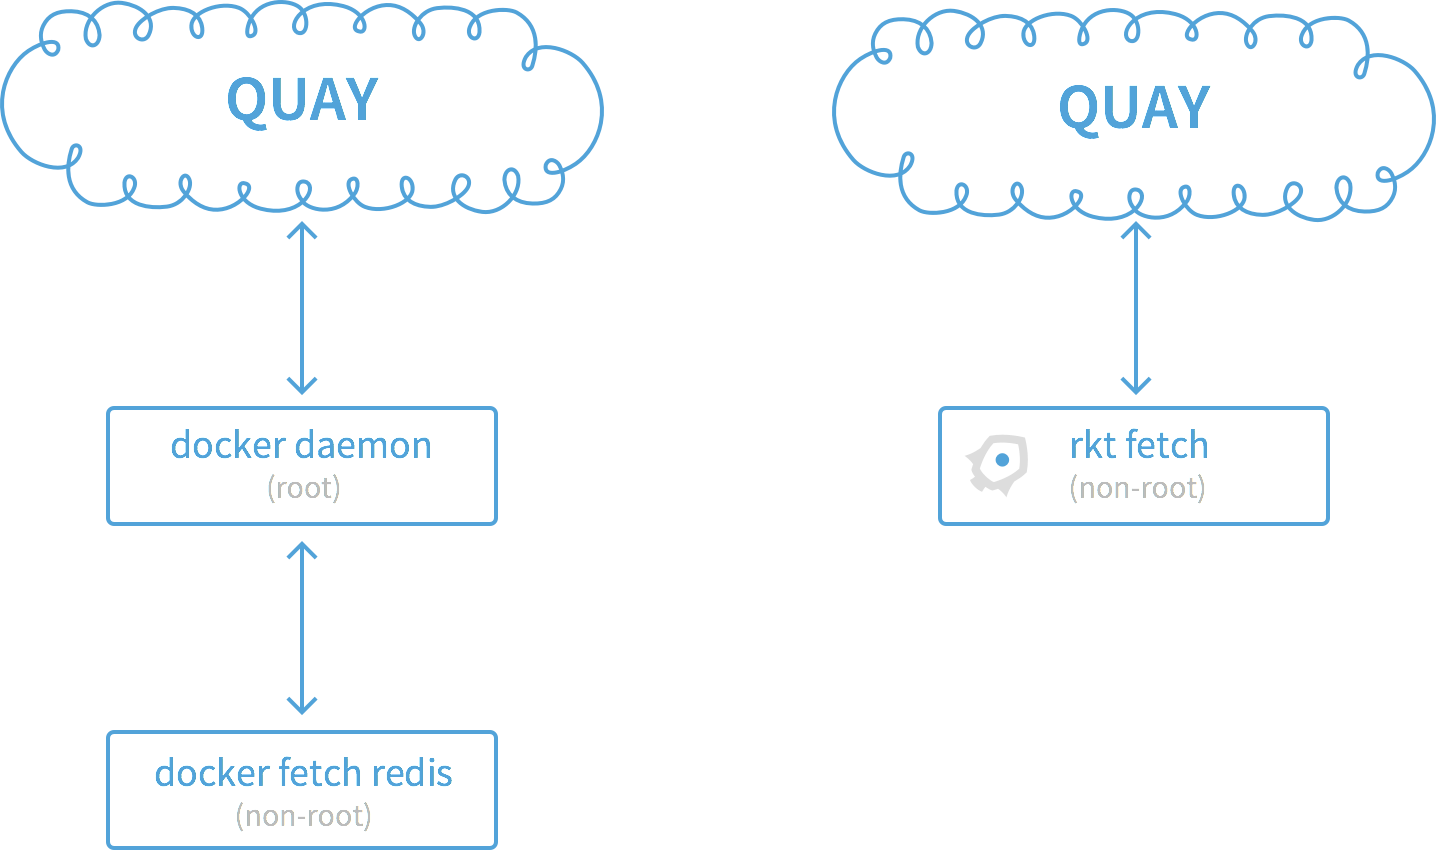
\includegraphics[width=0.75\textwidth]{rkt-vs-docker-fetch}
    \end{center}
\end{frame}

\begin{frame}{How does rkt compare to docker?}
    docker works with:
    \begin{itemize}
        \item The docker spec
    \end{itemize}
    \pause
    \vspace{1em}
    rkt works with:
    \begin{itemize}
        \item The docker spec
        \item The AppC spec
        \item The OCI image spec
    \end{itemize}
\end{frame}

\begin{frame}{How does rkt compare to docker?}
    rkt was designed with pods in mind.
    \begin{itemize}
        \item Running an image is running a pod with one app
        \item rkt can also accept pod manifests
    \end{itemize}
\end{frame}

% Section: how does rkt work?

\begin{frame}
    Outline
    \begin{itemize}
        \item What are containers?
        \item What is rkt?
        \item How do I get rkt?
        \item How do I use rkt?
        \item \textbf{How does rkt compare to docker?}
        \item How does rkt work?
        \item How do I build rkt containers?
        \item How does rktnetes work?
    \end{itemize}
\end{frame}

\begin{frame}
    Outline
    \begin{itemize}
        \item What are containers?
        \item What is rkt?
        \item How do I get rkt?
        \item How do I use rkt?
        \item How does rkt compare to docker?
        \item \textbf{How does rkt work?}
        \item How do I build rkt containers?
        \item How does rktnetes work?
    \end{itemize}
\end{frame}

\begin{frame}{How does rkt work?}
    When a pod is run with rkt, there are three stages to this.
\end{frame}

\begin{frame}{How does rkt work?}
    stage0:
    \begin{itemize}
        \item fetches images
        \item verifies images
        \item manages the image store
        \item manages overlayfs mounts
    \end{itemize}
\end{frame}

\begin{frame}{How does rkt work?}
    stage1:
    \begin{itemize}
        \item sets up isolation
        \item manages application mounts
        \item manages application networks
        \item starts application hypervisor
    \end{itemize}
\end{frame}

\begin{frame}{How does rkt work?}
    stage2:
    \begin{itemize}
        \item Your app!
    \end{itemize}
\end{frame}

\begin{frame}{How does rkt work?}
    The stage1 is pluggable! \\
    \pause
    \vspace{1em}
    Provided stage1s:
    \begin{itemize}
        \item coreos
        \item host
        \pause
        \item fly
        \pause
        \item kvm
    \end{itemize}
\end{frame}

% Section: how does rktnetes work?

% Section: how do I build rkt containers?

\begin{frame}
    Outline
    \begin{itemize}
        \item What are containers?
        \item What is rkt?
        \item How do I get rkt?
        \item How do I use rkt?
        \item How does rkt compare to docker?
        \item \textbf{How does rkt work?}
        \item How do I build rkt containers?
        \item How does rktnetes work?
    \end{itemize}
\end{frame}

\begin{frame}
    Outline
    \begin{itemize}
        \item What are containers?
        \item What is rkt?
        \item How do I get rkt?
        \item How do I use rkt?
        \item How does rkt compare to docker?
        \item How does rkt work?
        \item \textbf{How do I build rkt containers?}
        \item How does rktnetes work?
    \end{itemize}
\end{frame}

\begin{frame}{How do I build rkt containers?}
    acbuild: the App Container build system
    \begin{itemize}
        \pause
        \item Another cli tool
        \pause
        \item Install via GitHub release
        \pause
        \item Can create and modify ACIs
    \end{itemize}
\end{frame}

\begin{frame}{How do I build rkt containers?}
    Example 1: a static go binary
\end{frame}

\begin{frame}{How do I build rkt containers?}
    Example 2: nginx
\end{frame}

\begin{frame}
    Outline
    \begin{itemize}
        \item What are containers?
        \item What is rkt?
        \item How do I get rkt?
        \item How do I use rkt?
        \item How does rkt compare to docker?
        \item How does rkt work?
        \item \textbf{How do I build rkt containers?}
        \item How does rktnetes work?
    \end{itemize}
\end{frame}

\begin{frame}
    Outline
    \begin{itemize}
        \item What are containers?
        \item What is rkt?
        \item How do I get rkt?
        \item How do I use rkt?
        \item How does rkt compare to docker?
        \item How does rkt work?
        \item How do I build rkt containers?
        \item \textbf{How does rktnetes work?}
    \end{itemize}
\end{frame}

\begin{frame}{How does rktnetes work?}
    \begin{center}
        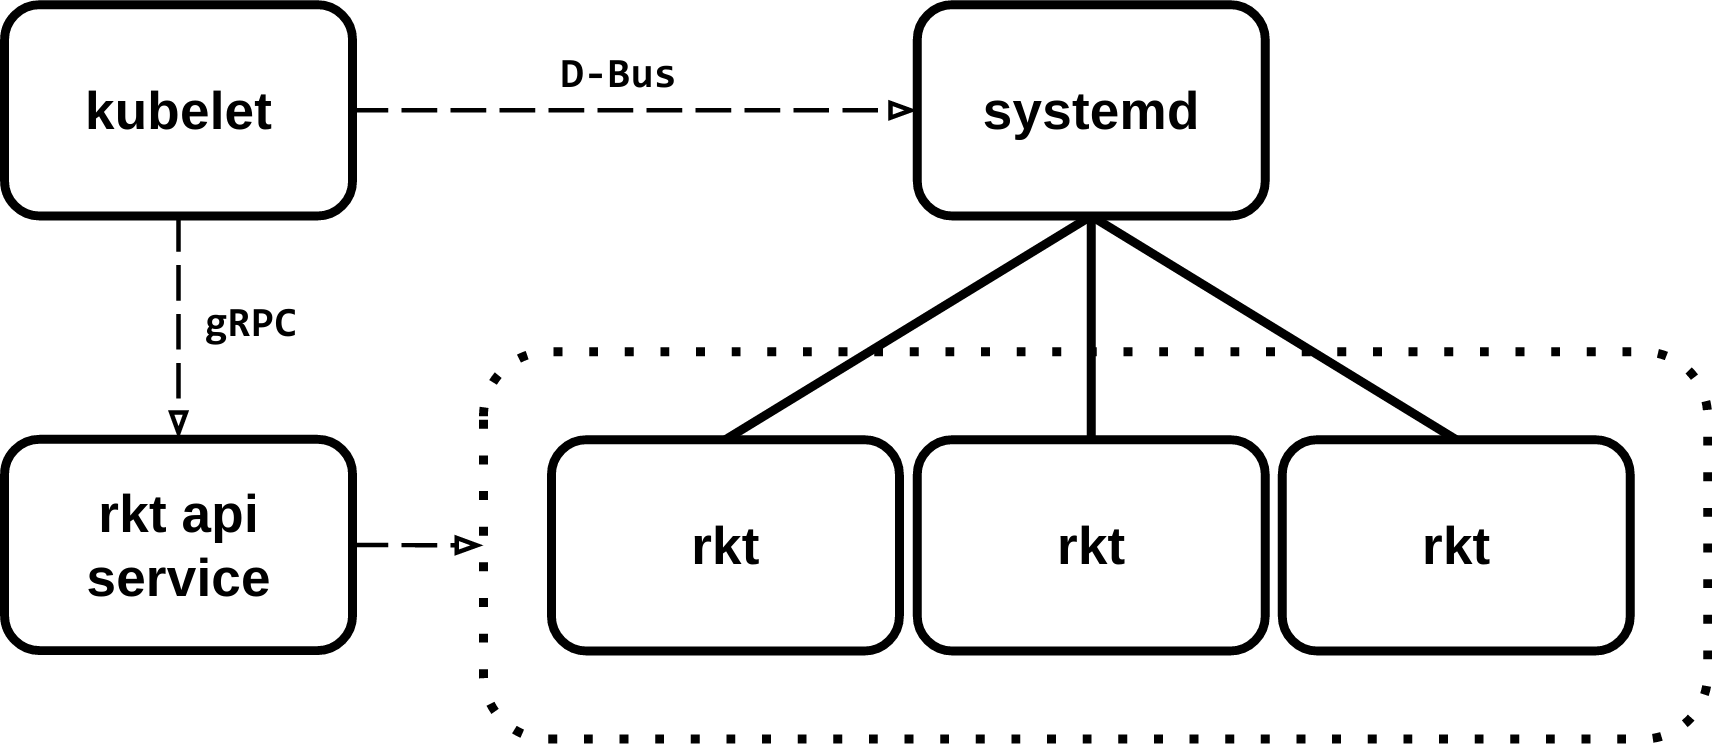
\includegraphics[width=0.75\textwidth]{rktnetes-model}
    \end{center}
\end{frame}

\begin{frame}
    \center \LARGE Questions? \normalsize
\end{frame}

\end{document}
